\chapter{Previous Work on Relationship Extraction}
In this chapter, we first introduce the most popular pre-trained models that are currently used in NLP. Then we discuss different metrics that are used on Relationship Extraction. Lastly, we research previous work done on the topic of training models for the relationship extraction task.

\section{NLP Models}
Lately, NLP tasks are dominated by solutions using pre-trained deep neural models with the transormer architecture. In this section, we introduce BERT, the first well-known model of this type that has set the trend.
\chybi{BERT, albert? + obecně asi transformer architektura}
\subsection{BERT}


\section{Metrics}
\todo{outdated}This section focuses on metrics in the Relationship extraction task, we first define those metrics and later discuss the pros and cons of each.

\subsection{Binary classification}

Let us start with metrics for binary classification. In binary classification, we are presented with an input vector and the goal is to determine whether the vector is of class A pro class B. Each prediction then falls into one of the following categories: correctly classified A input, correctly classified B input, wrongly classified A input as B, and a B input wrongly classified as A (Figure \ref{obr:CM}). 

\begin{figure}[h]\centering
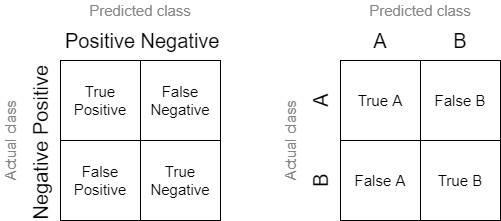
\includegraphics[width=140mm]{./img//Diplomka diagramy-Confusion matric}
\caption{Confusion matrix for binary classification}
\label{obr:CM}
\end{figure}

Another way to look at the same situation is to just predict whether an input is of class A or not. Those that way the prediction is a True / False value determining whether the model is of class A. This way, we can define the previously mentioned categories without using the specific classes as \defineterm{true positive} (TP), \defineterm{true negative} (TN), \defineterm{false negative} (FN) and \defineterm{false positive} (FP). Visualization of the result of classification on a dataset is called a \defineterm{confusion matrix}, we include such matrix\todo{without of the number of samples in each category} \ref{obr:CM}). We will use the abbreviations to represent the number of predictions that belong to the given category.  



\defineterm{Accuracy} expresses the ration between correct and incorrect predictions.
\begin{align}
Acc = \frac{TP+TN}{FP+FN}
\end{align} 



\defineterm{Precision} expresses the ratio correctly predicted positives within all predicted positives. Therefore, precision is a good metric if we want to avoid mistakenly classify falses as positives.

\begin{align} 
Prec = \frac{TP}{TP + FP}
\end{align}

\defineterm{Recall} is the complementary metric to precision. It expresses the ratio of all positives that were correctly predicted. In other words, it should be used when we need to find the maximum of positives in the data.

\begin{align}
Rec = \frac{TP}{TP + FN}
\end{align}

Let us show three use cases, each of the defined metrics will be the best fit in one case.

Suppose we have a collection of pictures of cats and dogs for adoption. If we were to classify pictures of cats and dogs based on the animal, we would most likely want to maximize the number of correct predictions. Accuracy would aim exactly for that.

If we knew that some adopters suffer from cynophobia (fear of dogs), suddenly the classifier should accommodate the fact by optimizing precision (where a cat is a positive). Note that precision (and recall) in binary classification will return different values if we swap which class is the positive and which is negative.

If the demand for cats extends supply and therefore we have more dogs than cats in the collection, searching for cats could get harder. In such a case, we would want to make sure that all cats are actually classified as cats, and recall would help with that.


To emphasize that the right choice of metric is significant suppose that we have balanced data (both true and false classes are equally represented). If our classifier just predicted that every input is positive, we would obtain the following: 0.5 accuracy, 0.5 precision, and 1 recall. If we were to predict all negatives accuracy and precision would remain 0.5 but recall suddenly drops to 0. If we were to randomly predict the result with even chances for both classes the expected results are 0.5 for all of those metrics. We just described three very different classifiers and the only thing we learned from accuracy and precision was that they were equally bad, without any insight about them. Recall in contrast successfully gave us insight about what the predictions likely are, but evaluated a bad classifier with the highest possible score.   

This whole section is in this thesis mostly to remind us that if we want to score well in a given metric, we will likely exploit the metric even if it might actually worsen our classifier. The choice of a metric for a task determines what gets optimized. Later in this section, we will debate such issues in our case, in the relationship extraction task.




F1

Often we might want a trade-off between being as precise as possible and recalling as much as possible. \defineterm{F1 score} is a harmonic mean of precision and recall (scaled to range from 0 to 1): \begin{align}
F1 = 2\frac{Prec \dot Rec}{Prec + Rec}
\end{align}and is quite widely used in competition tasks.

\subsection{Multiclass classification}


We already run into issues with asymmetry of precision and recall in binary classification (it is dependent on which class is chosen to be the positive one). We can address this by creating metrics per class. In the previous example about binary pet classification, we would get two sets of metrics, each describing the ability of the classifier to recognize given class apart from the rest.

Now we can easily extend this per class approach to multiclass classification. The formulas will remain exactly the same, only the way we obtain the TP, FP, TN, and FN values is a little different. In a sense nothing changed - if we imagine that the classifier is still binary then the situation is exactly the same. But if we compute those values out of confusion matrix (for class B) than TP is the value on position [B, B], FP is the sum of all in column B without TP, FN the sum of the row B without TP and the sum of cells outside of the Bth row and column are the TN. (Figure \ref{obr:BigCM})



\begin{figure}[h]\centering
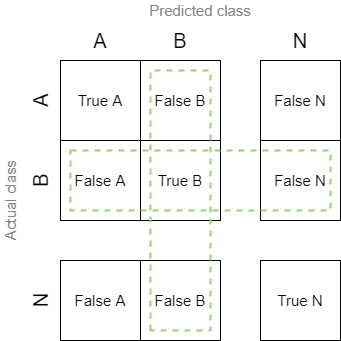
\includegraphics[width=80mm]{./img//Diplomka diagramy-Big Confusion matric}
\caption{Confusion matrix for N-class classification}
\label{obr:BigCM}
\end{figure}






As a solid way of examining the quality of the classifier, one could simply look at the confusion matrix and at all the per-class metrics. Although this would be insightful, it is not the most practical in terms of a clear comparison of two classifiers. Ideally, we aim for a metric or metrics that are as descriptive and comprehensive as possible but define an ordering of the classifiers.

Intuitively we will minimize the number of metrics by combining them into one value. To do so, we should acknowledge that the dataset we evaluate the performance of a classifier and a metric on needs to be taken into consideration.

An ideal dataset would be perfectly balanced. In real life we encounter two types of imbalance in datasets:

class representation distribution (CRD) is not uniform - classes are not equally represented 
class representation distribution is different in the test and the train part of the dataset

The second imbalance is tricky. Often, when optimizing the classifier, we do not know the CRD of the test dataset. We will therefore mostly focus on the first one. 


\subsubsection{Macro-averaged metrics}

The first method that comes to mind when we aim to combine the same metric of multiple classes into one, is the arithmetic mean. In most libraries and papers the term macro-[metric] (macro-recall, macro-F1, etc.) is used.  Macro averaged metrics tend to be the easy option that is used without much thought. So much so, that even though two macro-F1s are being used, often the exact formula is not included in papers. (The more common formula is the arithmetic mean of classes F1s, but the less often formula where the F1 is computed from macro-recall and macro-precision is also used \cite{Opitz2019MacroFA}.)

\subsubsection{Weight-averaged metrics}
If we aimed to pretty much just maximize a metric ignoring the class, instead of averaging the classes with the same weight, we would wight them by their \defineterm{support}. \chybi{co je support}

\chybi{vzorec}

\subsection{Relationship extraction metrics}
Whether or not to use macro metrics depends deeply on the use case and the dataset. In our case, the datasets tend to be very imbalanced (the majority of data are negative mentions, and even within the positive mentions the classes are highly unbalanced). This often leads to the idea of computing the combined metric only from positive classes.

\chybi{přehled co se běžně uvádí u kterého datasetu}

\chybi{problémy s tím, že CERED je sice taky nevyvážený, ale dost jinak}





\section{Relationship Extraction Models}

\chybi{matching the blanks}

\chybi{další články}
